\documentclass[10pt]{article}
\usepackage[polish]{babel}
\usepackage[utf8]{inputenc}
\usepackage[T1]{fontenc}
\usepackage{graphicx}
\usepackage[export]{adjustbox}
\graphicspath{ {./images/} }
\usepackage{amsmath}
\usepackage{amsfonts}
\usepackage{amssymb}
\usepackage[version=4]{mhchem}
\usepackage{stmaryrd}

\title{Akademia \\
 Pomorska \\
 w Stupsku }

\author{}
\date{}


\begin{document}
\maketitle
\begin{center}

\includegraphics[max width=\textwidth]{2024_11_21_1bed3b49e20da7fb8c35g-1}
\end{center}

\begin{center}

\includegraphics[max width=\textwidth]{2024_11_21_1bed3b49e20da7fb8c35g-1(1)}
\end{center}

\section*{LIGA MATEMATYCZNA \\
 im. Zdzisława Matuskiego \\
 FINAŁ 21 kwietnia 2022 \\
 SZKOEA PODSTAWOWA \\
 klasy IV - VI}
\section*{ZADANIE 1.}
Ania chce ułożyć kod do swojej szafki w szatni składający się z czterech cyfr dopisując do liczby 77 jedną cyfrę z lewej i jedną cyfrę z prawej strony w taki sposób, aby otrzymana liczba czterocyfrowa dzieliła się przez 18. Ile jest takich kodów? Podaj wszystkie możliwości.

\section*{ZADANIE 2.}
Adam zapisał liczbę za pomocą pięciu dziewiątek. Następnie dodał dwie pierwsze cyfry (licząc od lewej), zmazał je i w ich miejsce wpisał otrzymaną sumę. Potem to samo zrobił z nową liczbą i powtarzał tę czynność z każdą kolejną uzyskaną liczbą tak długo, aż pojawiła się liczba jednocyfrowa. Ile razy Adam wykonał opisaną operację zamiany pierwszych dwóch cyfr liczby na ich sumę?

\section*{ZADANIE 3.}
Wyznacz cztery kolejne liczby parzyste mające tę własność, że suma dwóch mniejszych jest mniejsza od 1000, a suma dwóch większych jest większa niż 1000. Podaj wszystkie możliwości.

\section*{ZADANIE 4.}
Bartek rzucał dwadzieścia razy sześcienną kostką do gry. Jedno oczko wypadło dwukrotnie rzadziej niż dwójka, ale trzy razy częściej niż trójka. Cztery oczka wypadły tyle samo razy co dwójka, a pięć oczek tyle samo razy co trzy oczka. Ile razy wypadło sześć oczek?

\section*{ZADANIE 5.}
Bok kwadratu \(A\) ma długość 10, a bok kwadratu \(B\) ma długość 20. Pomiędzy te kwadraty wstawiono kwadrat \(C\) tak, jak na rysunku. Oblicz obwód otrzymanej figury.\\
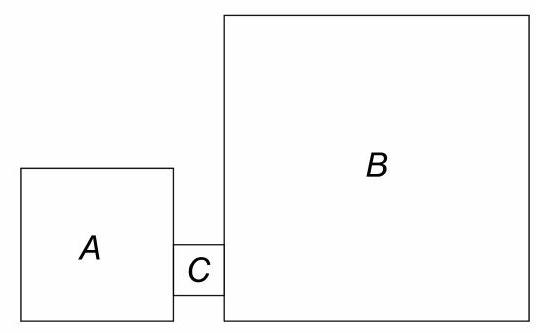
\includegraphics[max width=\textwidth, center]{2024_11_21_1bed3b49e20da7fb8c35g-1(2)}


\end{document}